\chapter{Experiment s krátkou trasou a dlhým vozidlom}\label{shortDlongV}

\begin{figure}[h]
  \centering
  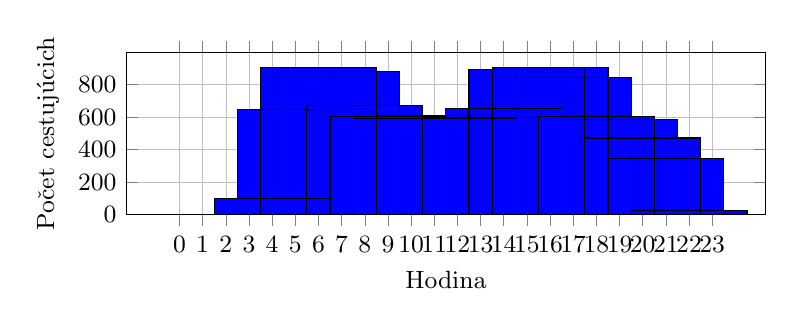
\begin{tikzpicture}
    \begin{axis}[
      width=0.8\textwidth,
      height=0.3\textwidth,
      xlabel={Hodina},
      ylabel={Počet cestujúcich},
      ymin=0,
      xtick={0,1,...,23},
      grid=both,
      major grid style={line width=.2pt,draw=gray!50},
      minor grid style={line width=.1pt,draw=gray!20},
      tick label style={font=\small},
      label style={font=\small},
      legend style={font=\small, at={(0.5,-0.2)}, anchor=north, legend columns=-1},
      ybar,
      bar width=5,
      ]
      \addplot[fill=blue] coordinates {
        (0, 0) (1, 0) (2, 0) (3, 0) (4, 101) (5, 647) (6, 907) (7, 883) 
        (8, 671) (9, 606) (10, 591) (11, 608) (12, 592) (13, 597) 
        (14, 654) (15, 893) (16, 905) (17, 845) (18, 602) (19, 584) 
        (20, 471) (21, 346) (22, 25) (23, 0)
      };
    \end{axis}
  \end{tikzpicture}
  \caption{Počet cestujúcich prichádzajúcich na zastávku za hodinu}
\end{figure}

\begin{figure}[h]
  \centering
  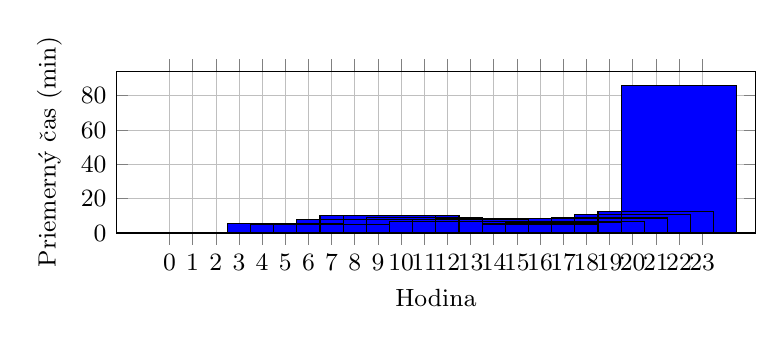
\begin{tikzpicture}
    \begin{axis}[
      width=0.8\textwidth,
      height=0.3\textwidth,
      xlabel={Hodina},
      ylabel={Priemerný čas (min)},
      ymin=0,
      xtick={0,1,...,23},
      grid=both,
      major grid style={line width=.2pt,draw=gray!50},
      minor grid style={line width=.1pt,draw=gray!20},
      tick label style={font=\small},
      label style={font=\small},
      legend style={font=\small, at={(0.5,-0.2)}, anchor=north, legend columns=-1},
      ybar,
      bar width=5,
      ]
      \addplot[fill=blue] coordinates {
        (0, 0) (1, 0) (2, 0) (3, 0) (4, 0) (5, 5.576506955177743) (6, 4.976846747519295) 
        (7, 5.1551528878822195) (8, 7.949329359165425) (9, 10.173267326732674) 
        (10, 9.981387478849408) (11, 8.924342105263158) (12, 6.70777027027027) 
        (13, 7.882747068676717) (14, 8.241590214067278) (15, 6.698768197088466) 
        (16, 5.232044198895028) (17, 5.972781065088758) (18, 6.714285714285714) 
        (19, 8.743150684931507) (20, 10.849256900212314) (21, 12.372832369942197) 
        (22, 85.8) (23, 0)
      };
    \end{axis}
  \end{tikzpicture}
  \caption{Priemerný čas strávený čakaním za hodinu}
\end{figure}

\begin{table}[h]
  \centering
  \begin{tabular}{|l|c|}
    \hline
    \textbf{Zastávka} & \# \\ \hline
    Lesná, Haškova & 0 \\ \hline
    Brechtova & 1 \\ \hline
    Blažkova & 2 \\ \hline
    Arbesova & 3 \\ \hline
    Heleny Malířové & 4 \\ \hline
    Lesná, nádraží & 5 \\ \hline
    Štefánikova čtvrť & 6 \\ \hline
    Provozníkova & 7 \\ \hline
    Lesnická & 9 \\ \hline
    Zemědělská & 10 \\ \hline
    Černá Pole, Erbenova & 11 \\ \hline
  \end{tabular}
  \caption{Rozpis zastávok}
\end{table}

\begin{table}[h]
  \centering
  \begin{tabular}{|c|l|}
    \hline
     \textbf{h} & \textbf{Odchody} \\ \hline
     05 & 00, 10, 20, 30, 40, 50 \\ \hline
     06 & 00, 10, 20, 30, 40, 50 \\ \hline
     07 & 00, 10, 20, 30, 40, 50 \\ \hline
     08 & 00, 20, 40 \\ \hline
     09 & 00, 20, 40 \\ \hline
     10 & 00, 20, 40 \\ \hline
     11 & 00, 15, 30, 45 \\ \hline
     12 & 00, 12, 24, 36, 48 \\ \hline
     13 & 00, 20, 40 \\ \hline
     14 & 00, 15, 30, 45 \\ \hline
     15 & 00, 12, 24, 36, 48 \\ \hline
     16 & 00, 10, 20, 30, 40, 50 \\ \hline
     17 & 00, 12, 24, 36, 48 \\ \hline
     18 & 00, 15, 30, 45 \\ \hline
     19 & 00, 20, 40 \\ \hline
     20 & 00, 20, 40 \\ \hline
     21 & 00, 30 \\ \hline
     22 & 00 \\ \hline
  \end{tabular}
  \caption{Časový rozpis}
\end{table}
